 
\begin{thebibliography}{9}
	
	\bibitem{luu}
	Thomas Luu 2017
	\textit{Fermions and Computers}
	
	\bibitem{lieb}
	E. Lieb, F. Wu 2003
	\textit{The one-dimensional Hubbard model: A Reminiscence}
	
	\bibitem{tasaki} 
	H. Tasaki 1998
	\textit{The Hubbard model - An Introduction and selected rigorous Results}
	
	\bibitem{jafari}
	Seyed A. Jafari 2008
	\textit{Introduction to Hubbard Model and Exact Diagonalization}
	
	\bibitem{gabrielsson}
	Anders F. Gabrielsson 2011
	\textit{Quantum Monte Carlo Simulations of
		the Half-filled Hubbard Model}
	
	\bibitem{computational}
	Marcus Petschlies, Carsten Urbach \textit{Computational Physics}
	
	\bibitem{Hubbard}
	M. Machida et al. \textit{High Performance LOBPCG Method for Solving Multiple Eigenvalues of Hubbard Model: Efficiency of Communication Avoiding Neumann Expansion Preconditioner}
	
	\bibitem{Hubbard2}
	\textit{http://atomcool.rice.edu/research/3d-lattice/}
\end{thebibliography}
\clearpage
\section{Appendix A - Analytical diagonalization of the 2-site model}
The matrix for the Hubbard Hamiltonian in the basis of the 16 states $\ket{i}, i\in {1,...,16}$ shown in section \ref{analytic} reads\footnote{note that due to particle conservation the matrix splits up into smaller blocks of same particle number}
\begin{equation*}
	H=
\begin{pmatrix}
	0&0&0&0&0&0&0&0&0&0&0&0&0&0&0&0\\
	0&-U/2&0&0&-t&0&0&0&0&0&0&0&0&0&0&0\\
	0&0&-U/2&0&0&-t&0&0&0&0&0&0&0&0&0&0\\
	0&0&0&0&0&0&0&0&-t&-t&0&0&0&0&0&0\\
	0&-t&0&0&-U/2&0&0&0&0&0&0&0&0&0&0&0\\
	0&0&-t&0&0&-U/2&0&0&0&0&0&0&0&0&0&0\\
	0&0&0&0&0&0&0&0&-t&-t&0&0&0&0&0&0\\
	0&0&0&0&0&0&0&0&-U&0&0&0&0&0&0&0\\
	0&0&0&-t&0&0&-t&0&-U&0&0&0&0&0&0&0\\
	0&0&0&-t&0&0&-t&0&0&-U&0&0&0&0&0&0\\
	0&0&0&0&0&0&0&0&0&0&-U&0&0&0&0&0\\
	0&0&0&0&0&0&0&0&0&0&0&-U/2&0&-t&0&0\\
	0&0&0&0&0&0&0&0&0&0&0&0&-U/2&0&-t&0\\
	0&0&0&0&0&0&0&0&0&0&0&-t&0&-U/2&0&0\\
	0&0&0&0&0&0&0&0&0&0&0&0&-t&0&-U/2&0\\
	0&0&0&0&0&0&0&0&0&0&0&0&0&0&0&0
\end{pmatrix}
\end{equation*}
Diagonalization gives 
\begin{align*}
	H_D= \text{diag}\biggl(0,0,0,-U,-U,-U, -\frac{U}{2}+t, -\frac{U}{2}+t,-\frac{U}{2}+t,-\frac{U}{2}+t,\\,-\frac{U}{2}-t,-\frac{U}{2}-t,-\frac{U}{2}-t,-\frac{U}{2}-t,-\frac{U}{2}-\sqrt{\frac{U^2}{4}+4t^2},-\frac{U}{2}+\sqrt{\frac{U^2}{4}+4t^2}\biggr)
\end{align*}
with the set of eigenstates $\ket{n_i}$:
\begin{align*}
	\ket{n_1}&= \ket{1}\hspace{2cm}\\
	\ket{n_2}&=-\frac{1}{\sqrt{2}} \ket{4} + \frac{1}{\sqrt{2}}\ket{7} \hspace{2cm}\\
	\ket{n_3}&=-\frac{1}{\sqrt{2}} \ket{14} + \frac{1}{\sqrt{2}}\ket{7}\\
	\ket{n_4}&=-\frac{1}{\sqrt{2}} \ket{12} + \frac{1}{\sqrt{2}}\ket{13}\\ \hspace{2cm}
	\ket{n_5}&=\ket{11} \\
	\ket{n_6}&=-\frac{1}{\sqrt{2}} \ket{9} + \frac{1}{\sqrt{2}}\ket{10}\\
	\ket{n_7}&= \ket{8} \\
	\ket{n_8}&=-\frac{1}{2} \ket{12} - \frac{1}{{2}}\ket{13}  + \frac{1}{{2}}\ket{14}  + \frac{1}{{2}}\ket{15}\\
	\ket{n_9}&=-\frac{1}{\sqrt{2}} \ket{3} + \frac{1}{\sqrt{2}}\ket{6}\\
	\ket{n_{10}}&=-\frac{1}{\sqrt{2}} \ket{2} + \frac{1}{\sqrt{2}}\ket{5}\\
	\ket{n_{11}}&=\frac{1}{\sqrt{2}} \ket{3} + \frac{1}{\sqrt{2}}\ket{6}\\
	\ket{n_{12}}&=\frac{1}{\sqrt{2}} \ket{2} + \frac{1}{\sqrt{2}}\ket{5}\\
	\ket{n_{13}}&=\frac{1}{2} \ket{12} + \frac{1}{{2}}\ket{13}  + \frac{1}{{2}}\ket{14}  + \frac{1}{{2}}\ket{15}\\
	\ket{n_{14}}&= -\frac{2t}{D_-} \ket{4} -\frac{2t}{D_-} \ket{7} +\frac{2t(\frac{U}{2}+\sqrt{\frac{U^2}{4}+4t^2})}{D_-} \ket{9} +\frac{2t(\frac{U}{2}+\sqrt{\frac{U^2}{4}+4t^2})}{D_-} \ket{10}\\
	\ket{n_{15}}&= +\frac{2t}{D_+} \ket{4} +\frac{2t}{D_+} \ket{7} +\frac{2t(-\frac{U}{2}+\sqrt{\frac{U^2}{4}+4t^2})}{D_+} \ket{9} +\frac{2t(-\frac{U}{2}+\sqrt{\frac{U^2}{4}+4t^2})}{D_+} \ket{10}\\
	\ket{n_{16}}&=\ket{16}
\end{align*}
where 
\begin{equation*}
	D_{\pm}= \biggl(\frac{U}{2}\pm\sqrt{\frac{U^2}{4}+4t^2}\biggr)\sqrt{\biggl|\frac{\sqrt{8}t^2}{\frac{U^2}{4}+4t^2}\biggr|^2+2}
\end{equation*}
\clearpage
\noindent Finally the nonvanishing components of the annihilation operators $(a^{x}_\sigma)_{i,j}$ in matrix form are
\begin{equation*}
	(a^1_\downarrow)_{6,1}=(a^1_\downarrow)_{7,5}=(a^1_\downarrow)_{9,2}=(a^1_\downarrow)_{11,3}=(a^1_\downarrow)_{12,8}=(a^1_\downarrow)_{13,10}=(a^1_\downarrow)_{15,4}=(a^1_\downarrow)_{16,14}=1 
\end{equation*}
\begin{equation*}
	(a^1_\uparrow)_{5,1}=-(a^1_\uparrow)_{7,6}=(a^1_\uparrow)_{8,2}=(a^1_\uparrow)_{10,3}=(a^1_\uparrow)_{61}=-(a^1_\uparrow)_{12,9}=-(a^1_\uparrow)_{13,11}=-(a^1_\uparrow)_{16,15}=1
\end{equation*}
\begin{equation*}
	(a^2_\downarrow)_{3,1}=(a^2_\downarrow)_{4,2}=(a^2_\downarrow)_{10,5}=(a^2_\downarrow)_{11,6}=(a^2_\downarrow)_{13,7}=(a^2_\downarrow)_{14,8}=(a^2_\downarrow)_{15,9}=(a^2_\downarrow)_{16,12}=1
\end{equation*}
\begin{equation*}
	(a^2_\uparrow)_{6,1} =(a^2_\uparrow)_{2,1}=-(a^2_\uparrow)_{4,3}=(a^2_\uparrow)_{8,5}=(a^2_\uparrow)_{9,6}=(a^2_\uparrow)_{12,7}=-(a^2_\uparrow)_{14,10}=-(a^2_\uparrow)_{15,11}=-(a^2_\uparrow)_{16,13}=1
\end{equation*}

\section{Appendix B - Numerical calculation}
\subsection{Fermion matrix for $L=3$}\label{MM}
\scalebox{0.9}{
$
\left(\begin{array}{cccccccccccc}
	1 & 0 & 0 & e^{-\phi_{14}} & 0 & 0 & 0 & \tilde{t} & 0 & 0 & 0 & \tilde{t} \\
	-e^{-\phi_{11}} & 1 & 0 & 0 & -\tilde{t} & 0 & 0 & 0 & -\tilde{t} & 0 & 0 & 0 \\
	0 & -e^{-\phi_{12}} & 1 & 0 & 0 & -\tilde{t} & 0 & 0 & 0 & -\tilde{t} & 0 & 0 \\
	0 & 0 & -e^{-\phi_{13}} & 1 & 0 & 0 & -\tilde{t} & 0 & 0 & 0 & -\tilde{t} & 0 \\
	0 & 0 & 0 & \tilde{t} & 1 & 0 & 0 & e^{-\phi_{24}} & 0 & 0 & 0 & \tilde{t} \\
	-\tilde{t} & 0 & 0 & 0 & -e^{-\phi_{21}} & 1 & 0 & 0 & -\tilde{t} & 0 & 0 & 0 \\
	0 & -\tilde{t} & 0 & 0 & 0 & -e^{-\phi_{22}} & 1 & 0 & 0 & -\tilde{t} & 0 & 0 \\
	0 & 0 & -\tilde{t} & 0 & 0 & 0 & -e^{-\phi_{23}} & 1 & 0 & 0 & -\tilde{t} & 0 \\
	0 & 0 & 0 & \tilde{t} & 0 & 0 & 0 & \tilde{t} & 1 & 0 & 0 & e^{-\phi_{34}} \\
	-\tilde{t} & 0 & 0 & 0 & -\tilde{t} & 0 & 0 & 0 & -e^{-\phi_{31}} & 1 & 0 & 0 \\
	0 & -\tilde{t} & 0 & 0 & 0 & -\tilde{t} & 0 & 0 & 0 & -e^{-\phi_{32}} & 1 & 0 \\
	0 & 0 & -\tilde{t} & 0 & 0 & 0 & -\tilde{t} & 0 & 0 & 0 & -e^{-\phi_{33}} & 1
\end{array}\right)
$
}

\subsection{Additional plots}
\begin{figure}[H]
	\centering
	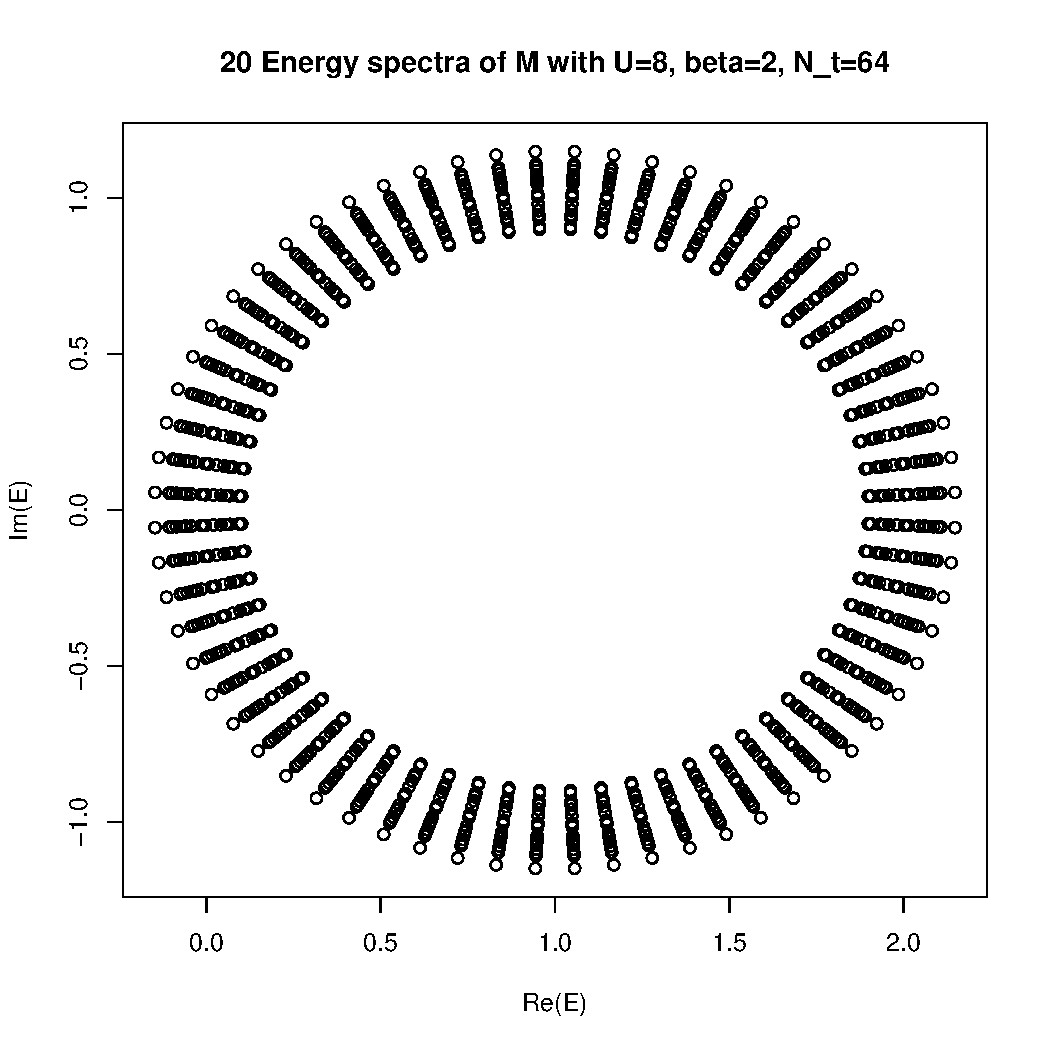
\includegraphics[width=0.5\linewidth]{figs/spectra}
	\caption[Energy Spectra]{Energy spectra for 20 sampled $\phi$, with $U=8$, $\beta=2$ and $N_t=64$}
	\label{fig:spectra}
\end{figure}
\begin{figure}[H]
	\centering
	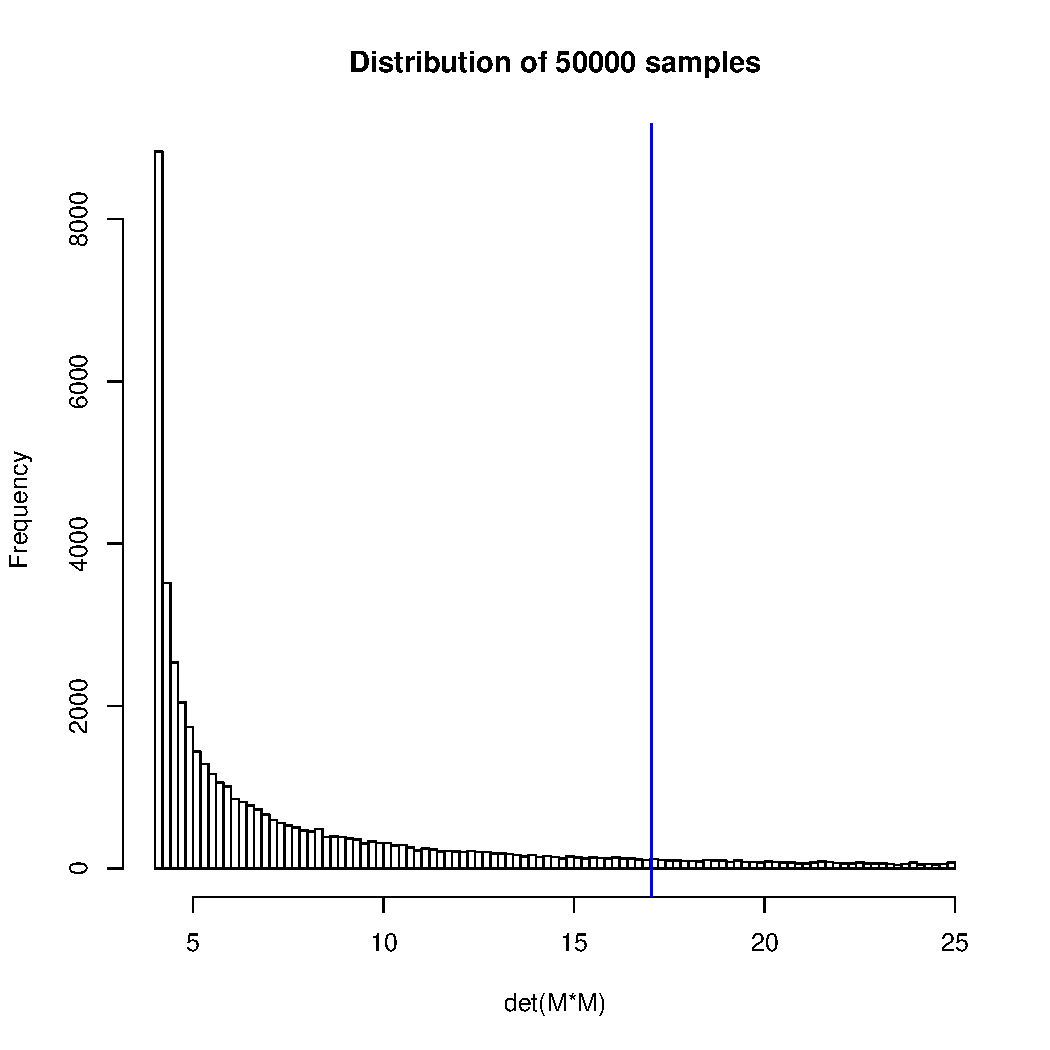
\includegraphics[width=0.5\linewidth]{figs/distribution}
	\caption[Distribution of 50000 samples]{This histogram shows the distribution of 50000 samples for a calculation of $Z$ for a 1 site lattice with $U=2$, $\beta=2$ and $N_t=24$. The blue line marks the mean, i.e. the result of the calculation. (Notice that the histogram was cut to focus on the interesting part)}
	\label{fig:distribution}
\end{figure}
\begin{figure}[H]
	\centering
	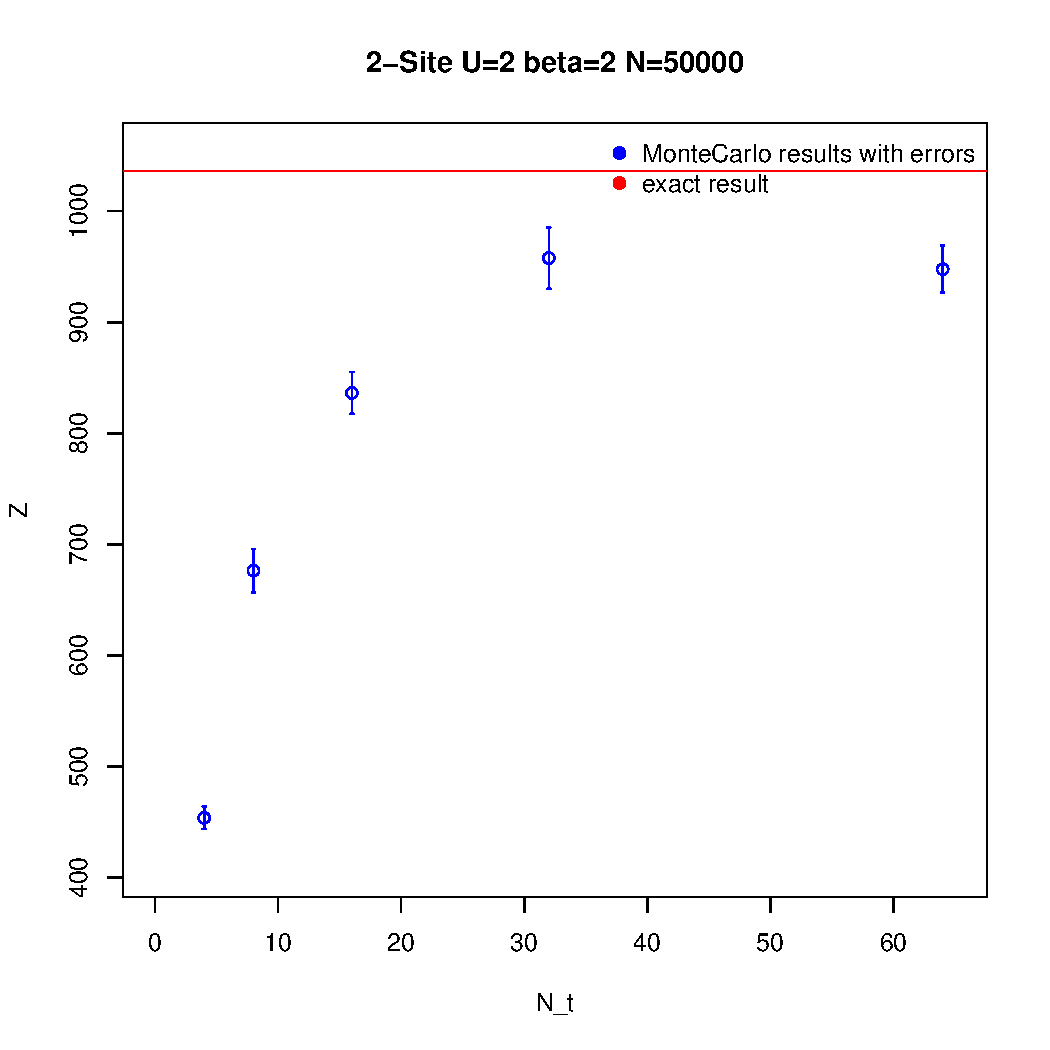
\includegraphics[width=0.5\linewidth]{figs/plot_Z2Nt}
	\caption[L2 Partition function]{The partition function of a 2-site lattice with $U=2$, $\beta=2$ and $N=50000$ for increasing $N_t$. The red line marks the exact value.}
	\label{fig:plotz2nt}
\end{figure}

\begin{figure}[H]
	\centering
	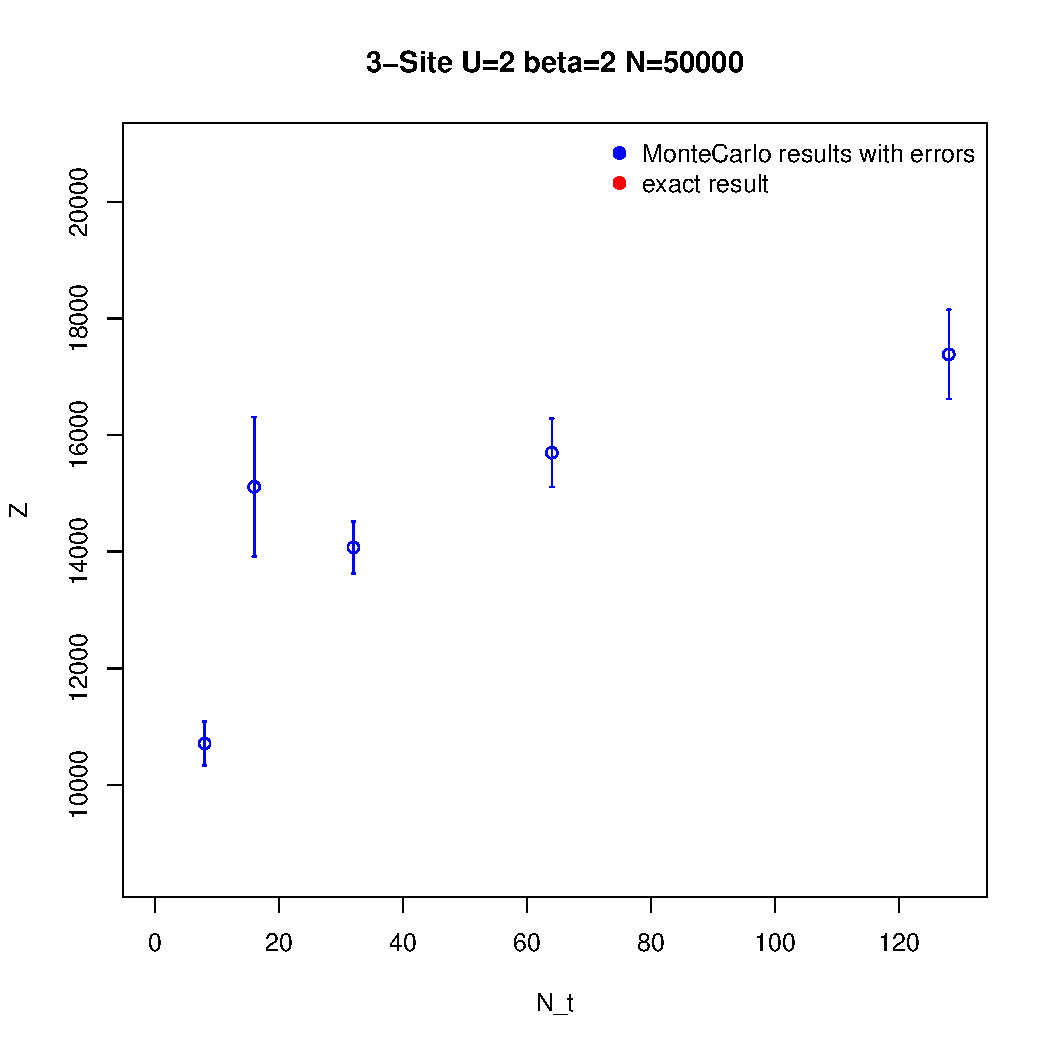
\includegraphics[width=0.5\linewidth]{figs/plot_Z3Nt}
	\caption[L3 Partition function]{The partition function of a 3-site lattice with $U=2$, $\beta=2$ and $N=50000$ for increasing $N_t$.}
	\label{fig:plotz3nt}
\end{figure}

\section{Appendix C - Additional Method}
\subsection{Metropolis-Hastings (failed attempt)}
The following method does not work for the Hubbard-Model, but since we spent a lot of time on it, we want to introduce it anyways.
The Metropolis-Hasting algorithm is a variant of Markov Chain Monte-Carlo where first an initial state of the system is randomly chosen.
For example the electron configuration of a lattice. Then the system gets repeatedly the chance to change its state by spin flips, electron hops, etc. This change will be, similarly to simulated annealing, accepted with a probability \eqref{acceptance} that depends on the energy difference that the change of state causes and the inverse temperature $\beta$.
\begin{equation}\label{acceptance}
p_{acceptance} = \min(1,\exp(-\beta*\Delta H))
\end{equation}
The resulting set of states is a weighted representation of the full system as it prefers physically favorable states.
Therefore the expectation value of an operator can be approximated by averaging over the result for each chosen state.
This method works well for the Ising-Model, however it can not be applied to the Hubbard-Model, which has no diagonal Hamiltonian and therefore non trivial eigenstates, which are superpositions of an exponentially large number of basisstates.
The energy(difference), which is crucial for the Metropolis algorithm, is hence not well defined for the different electron configurations.